% \usepackage{tikz}
% \usetikzlibrary{calc}


% \begin{figure}[htbp]
%     \centering

%     % Main figure
%     \begin{tikzpicture}[remember picture]
%         \node[inner sep=0] (mainplot) {%
%             \includegraphics[width=0.94\textwidth]{images/poisson_b1.png}
%         };

%         % Approximate location of the black zoom box
%         \coordinate (zoomsource) at
%             ($(mainplot.south west)!0.50!(mainplot.south east)+(0,3.1cm)$);
%     \end{tikzpicture}

%     \vspace{-0.1em}

%     % Bottom row
%     \begin{minipage}[t]{0.66\textwidth}
%         \vspace{-0.03pt}
%         \setlength{\abovecaptionskip}{0pt}
%         \caption{
%             Outer-refinement levels $k=0,3,6$ for
%             Algorithm~\ref{outerloop} applied to the
%             $\epsilon=0.2$ pseudospectrum of the Dirac-type operator
%             \eqref{dirac eig}. Black dots indicate the exact eigenvalues
%             \eqref{eigs dirac}. Red, blue, and green triangles are classified
%             as outside, inside, and on the pseudospectral contour,
%             respectively. White triangles outlined in grey remain active.
%             A magnified view of the $\mathcal{T}_6$ result over the region
%             $[1.7,2.3]\times[-0.3,0.3]$ is shown to the right, with the
%             desired contour indicated by the dashed purple circle.
%         }
%         \label{dirac results}
%     \end{minipage}
%     \hfill
%     \begin{minipage}[t]{0.30\textwidth}
%         \vspace{0pt}
%         \centering
%         \begin{tikzpicture}[remember picture]
%             \node[inner sep=0] (zoomplot) {%
%                 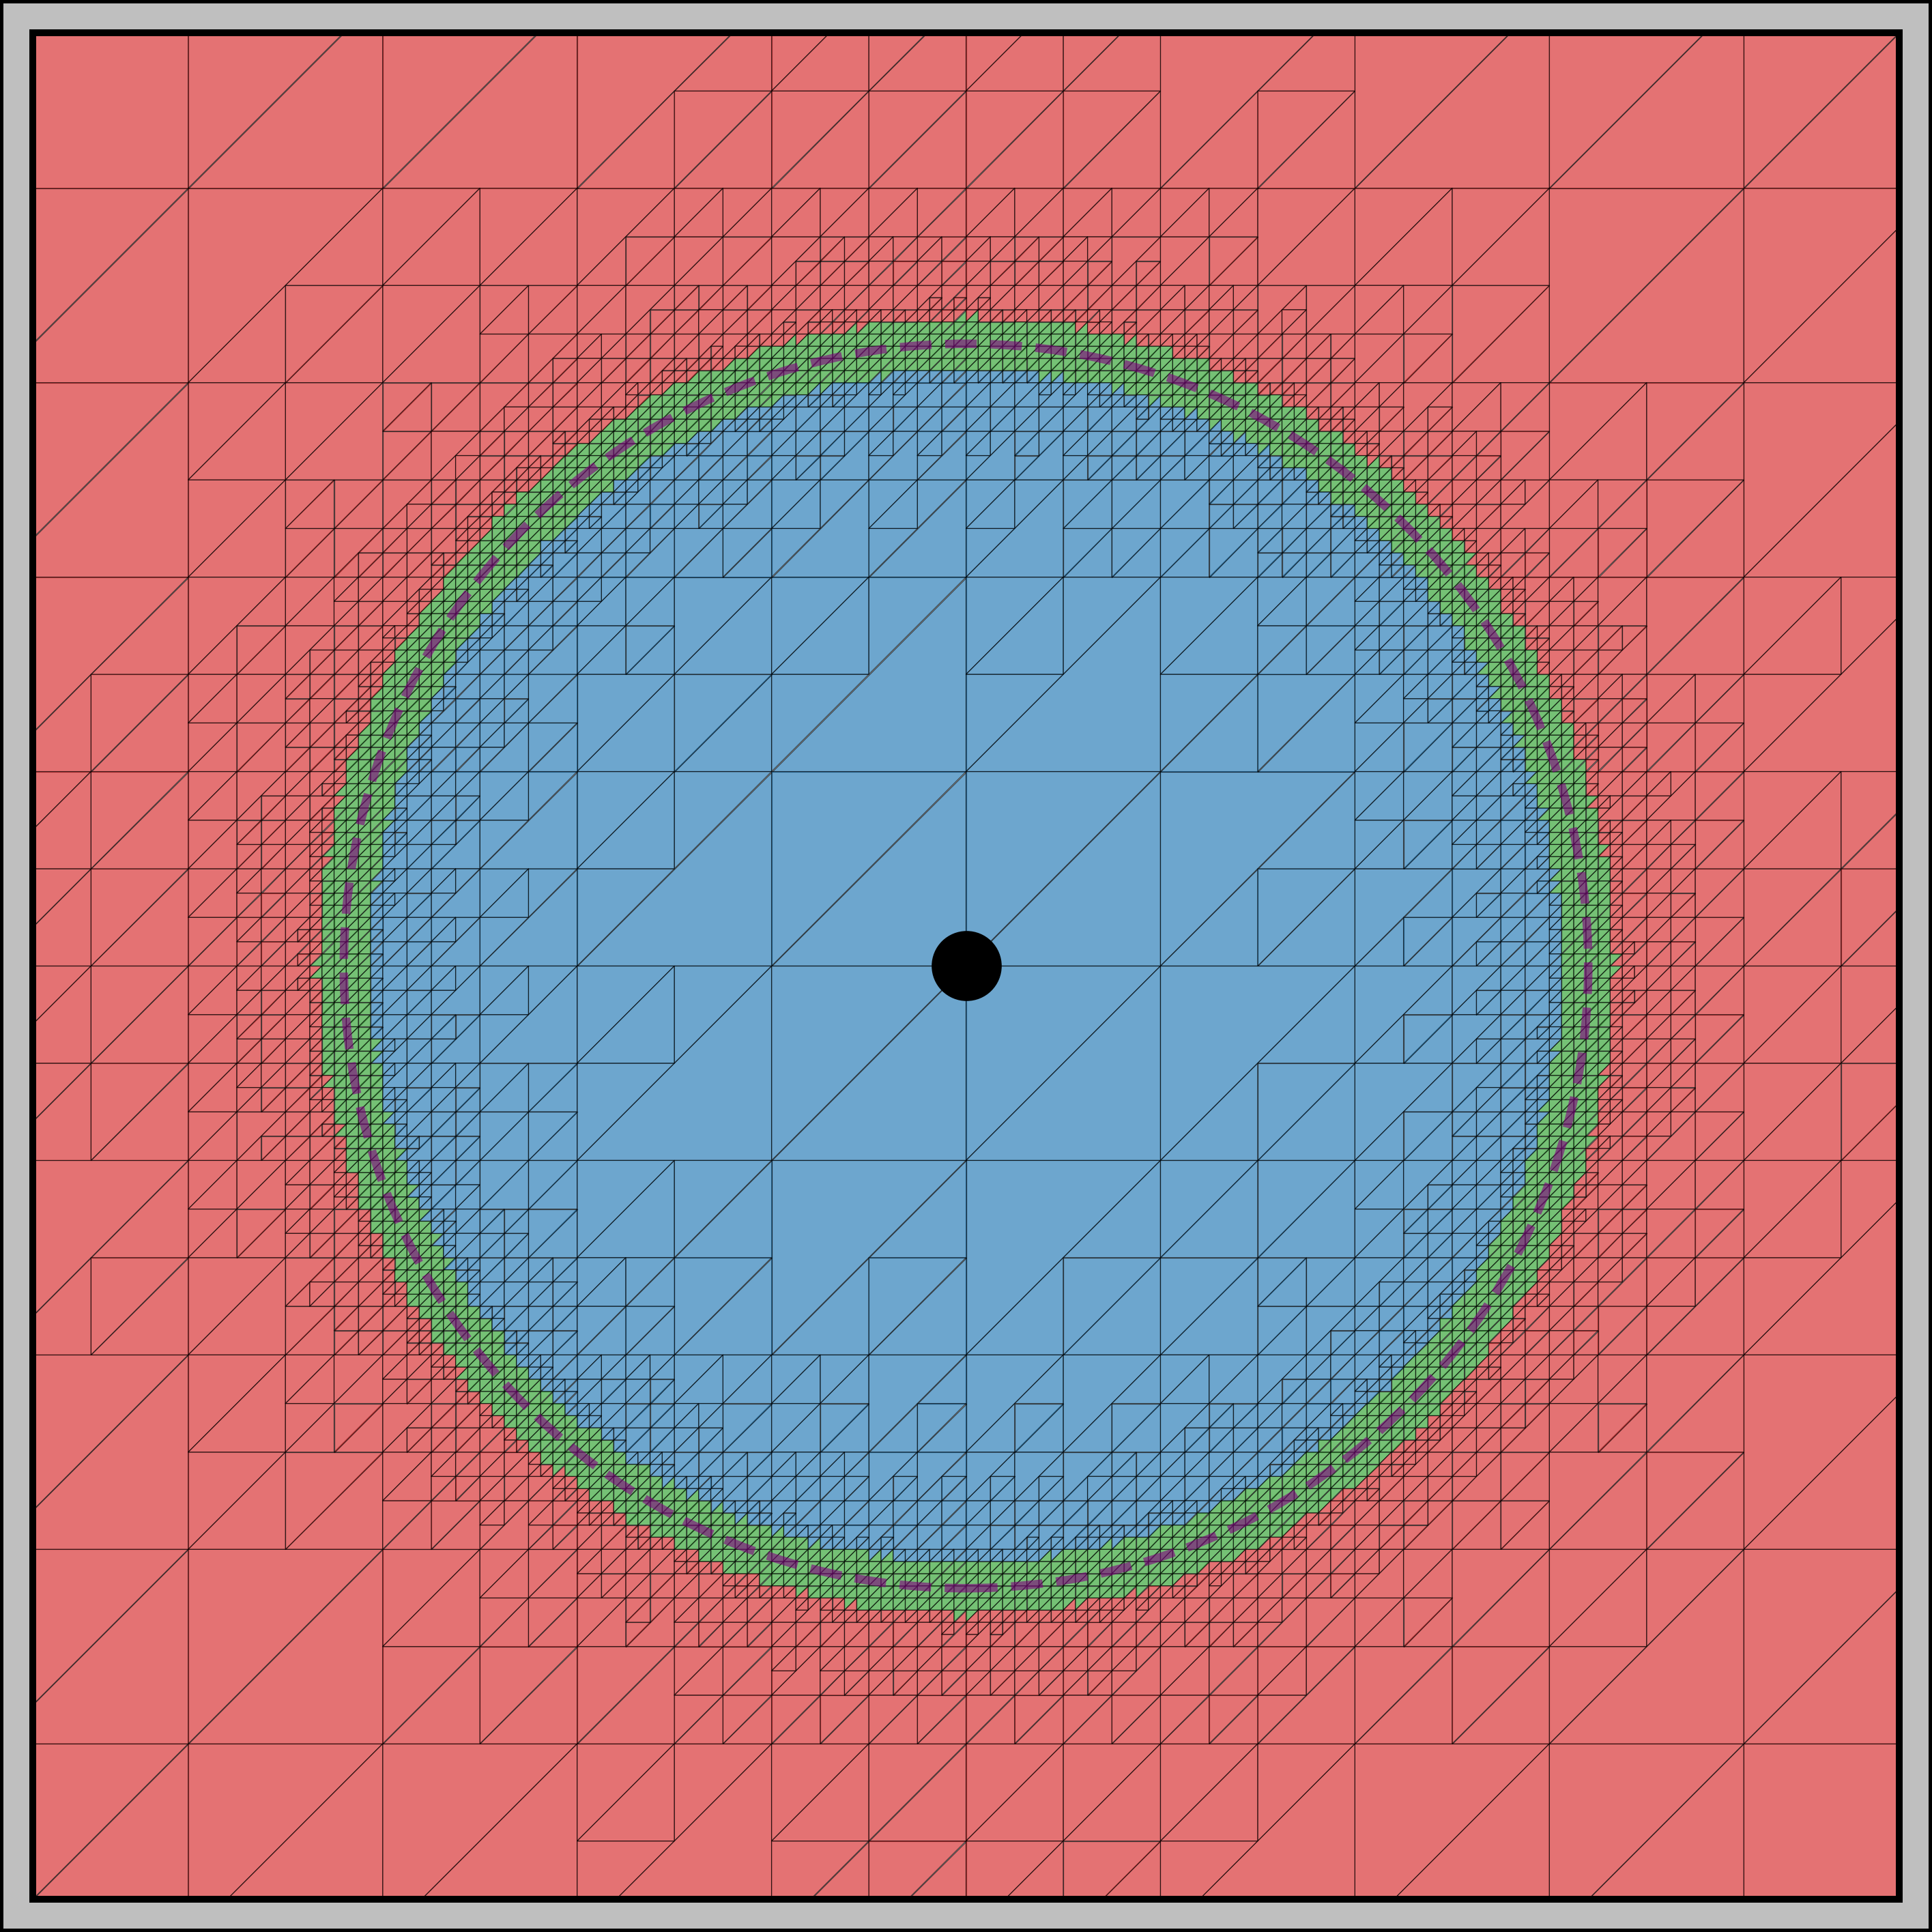
\includegraphics[width=\textwidth]{images/poisson_b2.png}
%             };
%         \end{tikzpicture}
%     \end{minipage}

%     % Arrow from boxed region to magnified view
%     \begin{tikzpicture}[remember picture,overlay]
%         \draw[->,thick]
%             (zoomsource)
%             .. controls +(2.0cm,-0.4cm) and +(-0.7cm,0.8cm) ..
%             (zoomplot.north west);
%     \end{tikzpicture}

% \end{figure}




% BEST SO FAR


\begin{figure}[htbp]
    \centering

    % Main figure
    \includegraphics[width=0.97\textwidth]{images/poisson_sweeps_combined.png}

    \vspace{-1.3em}

    % Bottom row
    \begin{minipage}[t]{0.67\textwidth}
        \vspace{-0.03pt}
        \setlength{\abovecaptionskip}{0pt}
        \caption[The Computed $\epsilon = 0.2$ Pseudospectral Picture for the One-Dimensional Dirac Operator]{Outer-refinement levels $k=0,3,6$ for
            \mbox{\Cref{outerloop}} applied to the  $\epsilon = 0.2$ pseudospectrum of the Dirac operator
            \eqref{dirac pois}. Black dots mark the exact eigenvalues
            \eqref{eigs dirac}. Red, blue, and green triangles are classified
            as outside, inside, and on the contour,
            respectively. White triangles are unclassified.
            A magnified view of the $\mathcal{T}_6$ result over
            $[1.7,2.3]\times[-0.3,0.3]$ is shown to the right, with the
            desired contour indicated by a purple dashed circle.
        }
        \label{dirac results}
    \end{minipage}
    \hfill
    \begin{minipage}[t]{0.30\textwidth}
        \vspace{4pt}
        \centering
        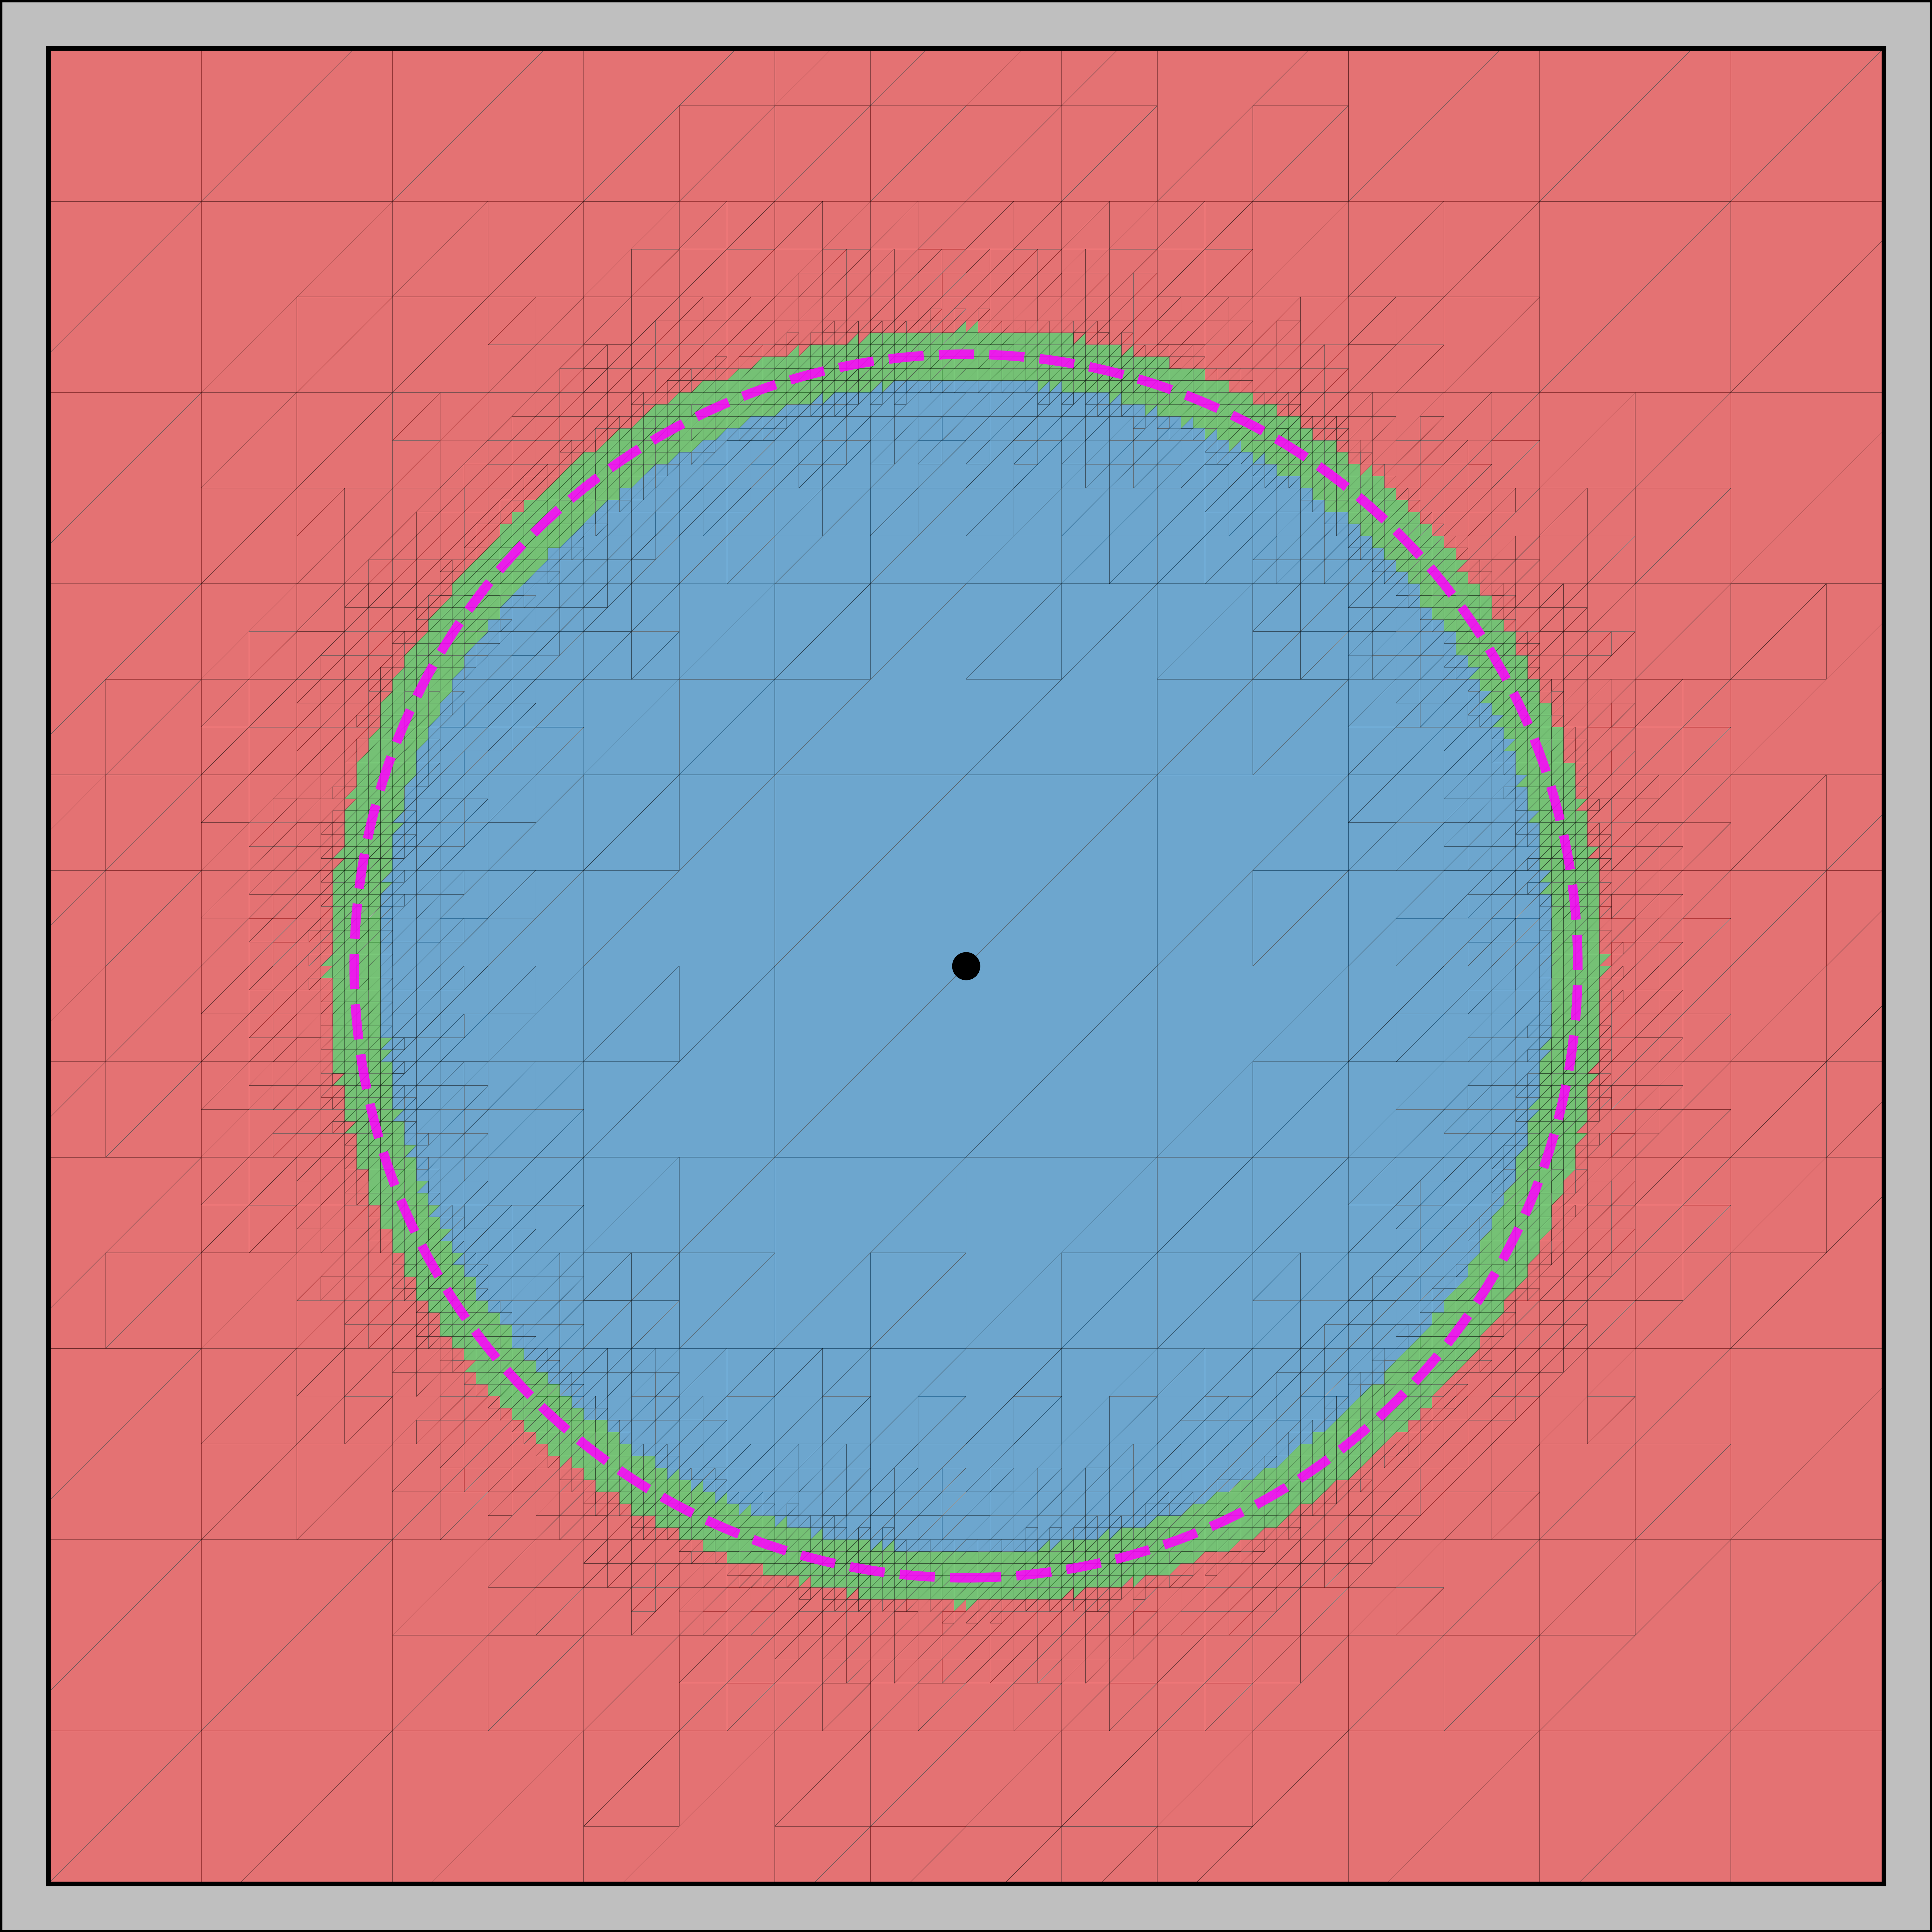
\includegraphics[width=0.95\textwidth]{images/poisson_zoom_standalone.png}
    \end{minipage}

\end{figure}





% \begin{figure}[htbp]
%     \centering

%     % Main figure
%     \includegraphics[width=0.95\textwidth]{images/poisson_sweeps_combined.png}

%     \vspace{-1.3em}

%     % Bottom row
%     \begin{minipage}[t]{0.67\textwidth}
%         \vspace{-0.03pt}
%         \setlength{\abovecaptionskip}{0pt}
%         \caption[The Computed $\epsilon = 0.2$ Pseudospectral Picture for the One-Dimensional Dirac Operator]{Outer-refinement levels $k=0,3,6$ for \mbox{\Cref{outerloop}} applied to the  $\epsilon = 0.2$ pseudospectrum of the Dirac operator
%             \eqref{dirac pois}. Black dots mark the exact eigenvalues
%             \eqref{eigs dirac}. Red, blue, and green triangles are classified
%             as outside, inside, and on the contour,
%             respectively. White triangles are unclassified.
%             A magnified view of the $\mathcal{T}_6$ result over
%             $[1.7,2.3]\times[-0.3,0.3]$ is shown to the right, with the
%             desired contour indicated by a purple dashed circle.
%         }
%         \label{dirac results}
%     \end{minipage}
%     \hfill
%     \begin{minipage}[t]{0.30\textwidth}
%         \vspace{6pt}
%         \centering
%         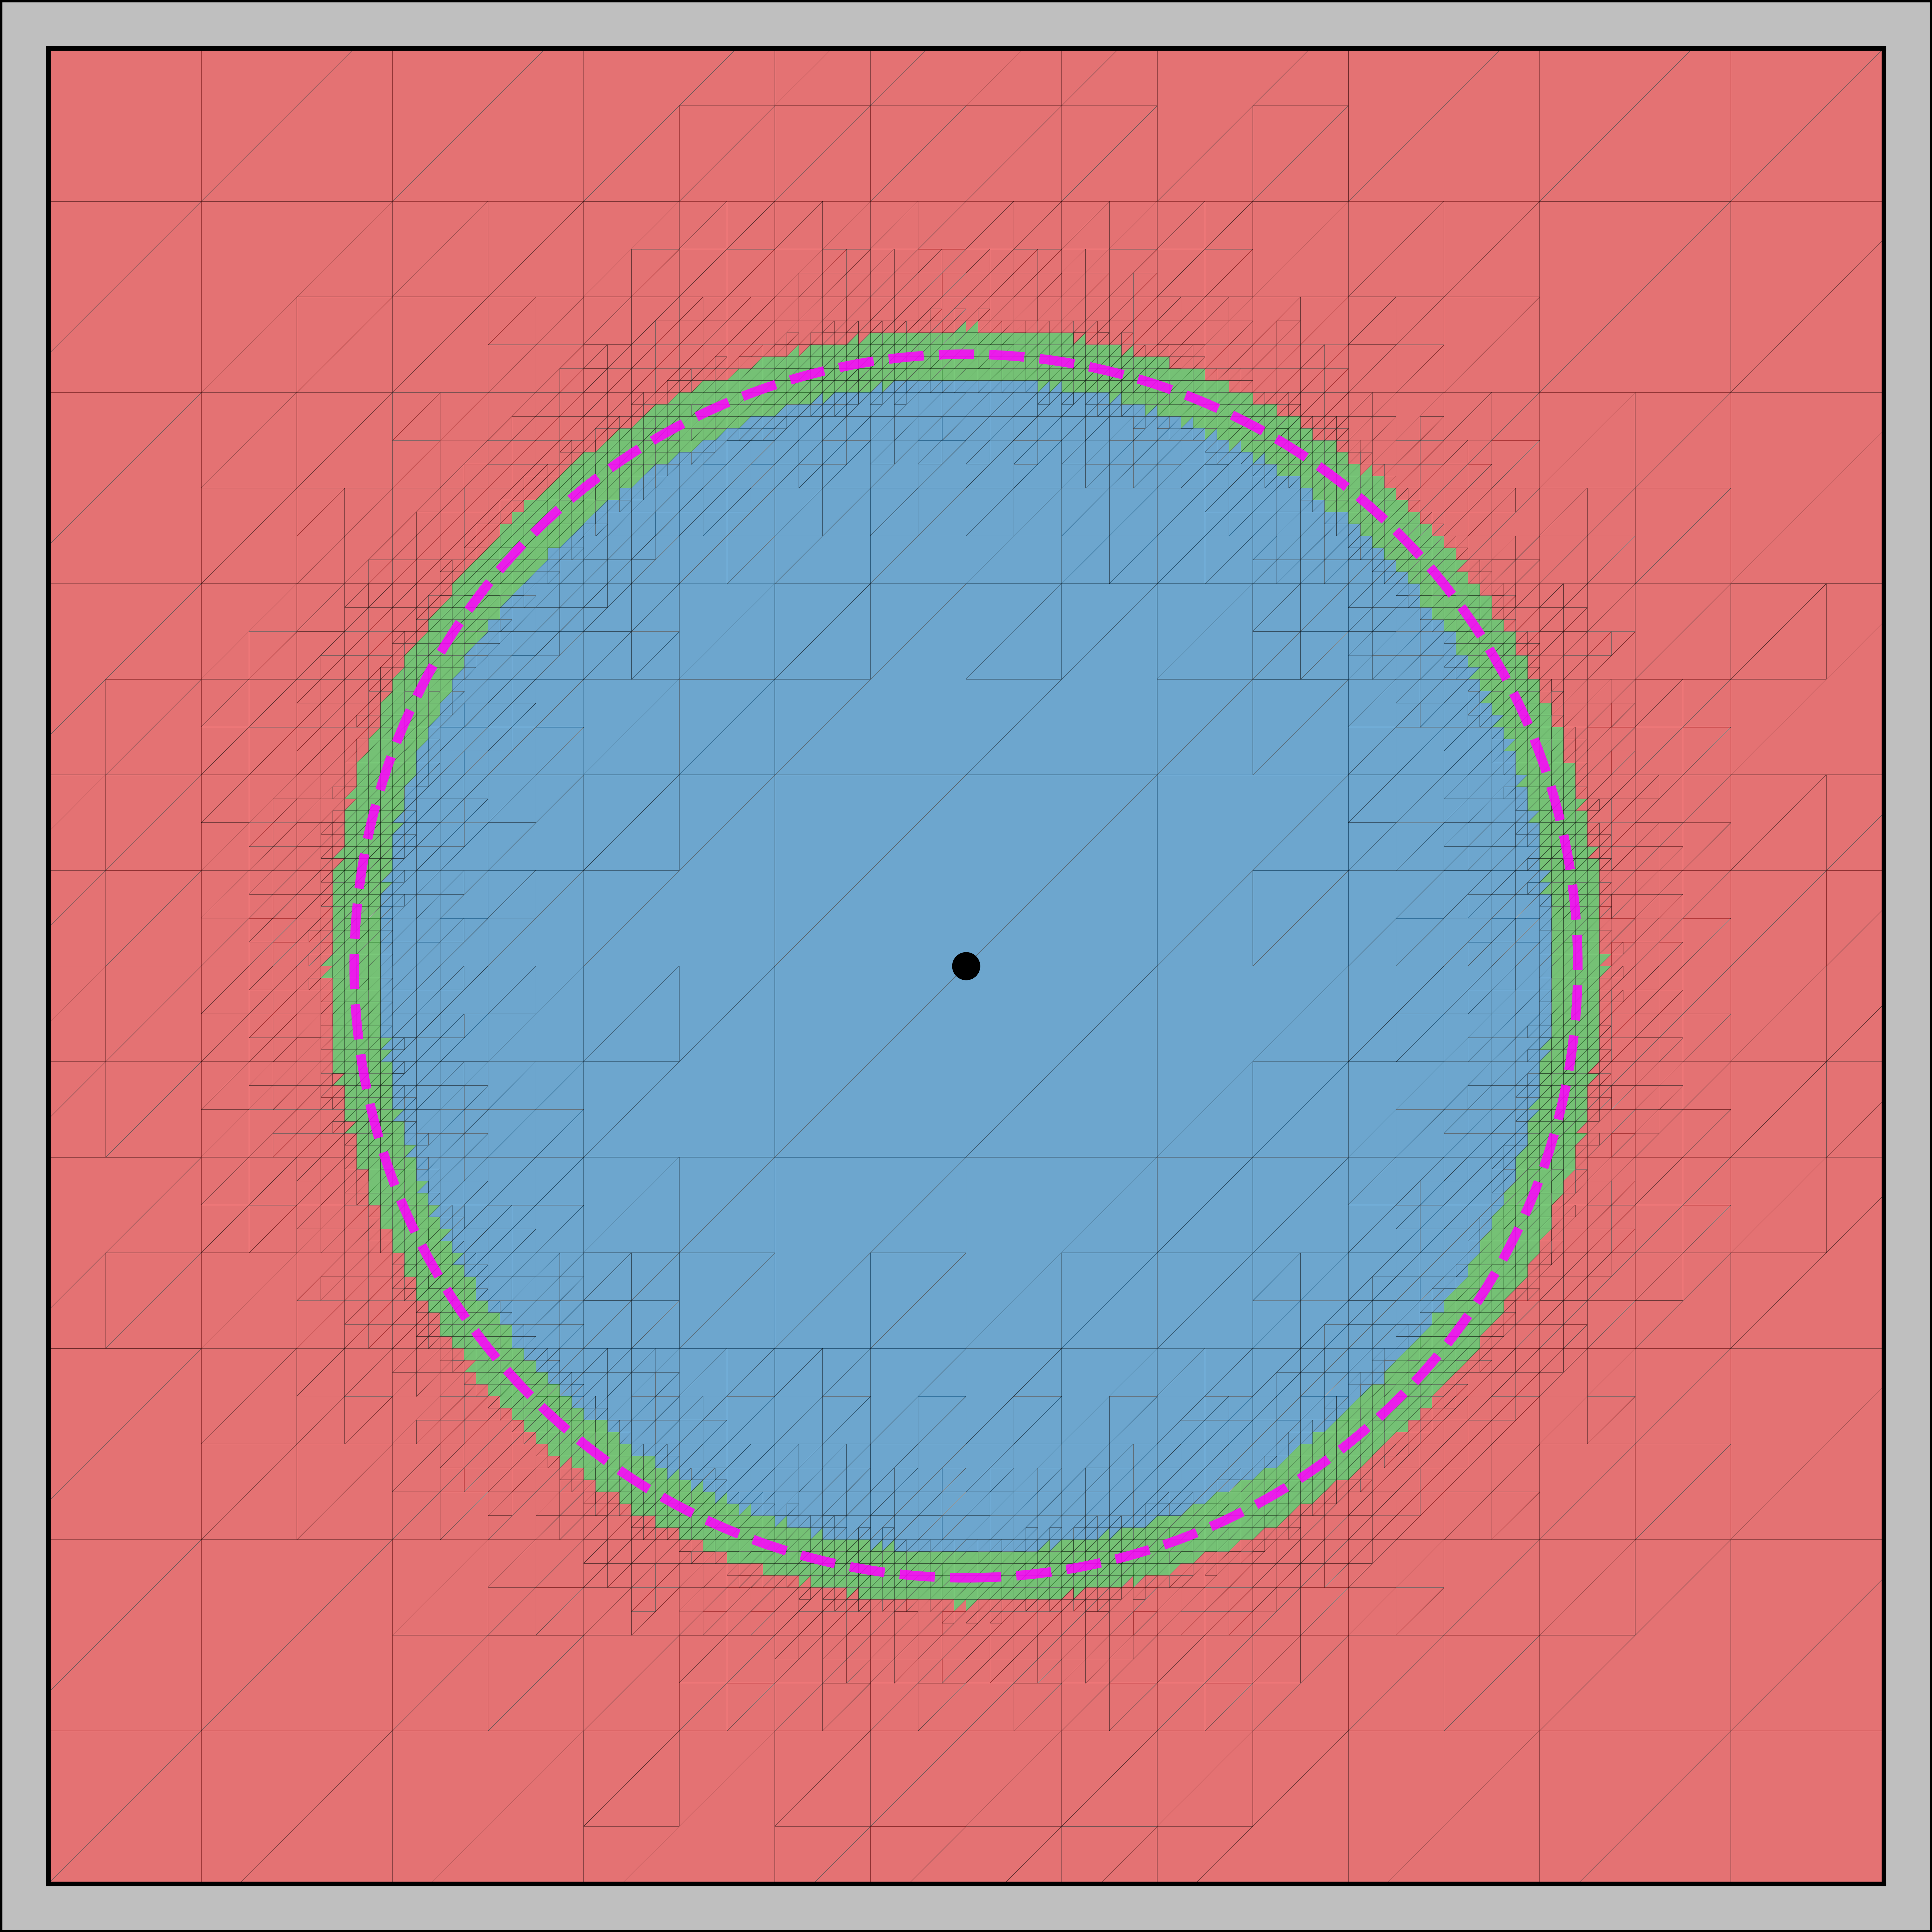
\includegraphics[width=1\textwidth]{images/poisson_zoom_standalone.png}
%     \end{minipage}

% \end{figure}










% \begin{figure}[htbp]
%     \centering

%     % Main figure
%     \includegraphics[width=\textwidth]{images/poisson_b1.png}

 

%     % Bottom row: text on left, zoom on right
%     \begin{minipage}[c]{0.62\textwidth}
%         \small
%         % Snapshots of Algorithm~\ref{outerloop} applied to the
%         % $\epsilon=0.2$ pseudospectrum of the Diract-type operator \eqref{dirac eig}. The black dots indicate the
%         % exact eigenvalues \eqref{eigs dirac}. Red triangles have been classified as
%         % outside the $\epsilon$-pseudospectrum, blue triangles as inside, green
%         % triangles as lying on the pseudospectral contour, and white triangles
%         % outlined in grey remain active. The resolution of the final sweep makes the green triangles hard to distinguish. We therefore present a magnified view.
%         \caption{Outer-refinement levels $k=0,3,6$ for
%         Algorithm~\ref{outerloop} applied to the
%         $\epsilon=0.2$ pseudospectrum of the Dirac-type operator
%         \eqref{dirac eig}. Black dots indicate the exact eigenvalues
%         \eqref{eigs dirac}. Red, blue, and green triangles are classified
%         as outside, inside, and on the pseudospectral contour,
%         respectively. White triangles outlined in grey remain active.
%        A magnified view of the $\mathcal{T}_6$ result over the region $[1.7,2.3]\times[-0.3,0.3]$ is shown to the right, with the desired contour indicated by the dashed purple circle.}
%     \end{minipage}
%     \hfill
%     \begin{minipage}[c]{0.32\textwidth}
%         \centering
%         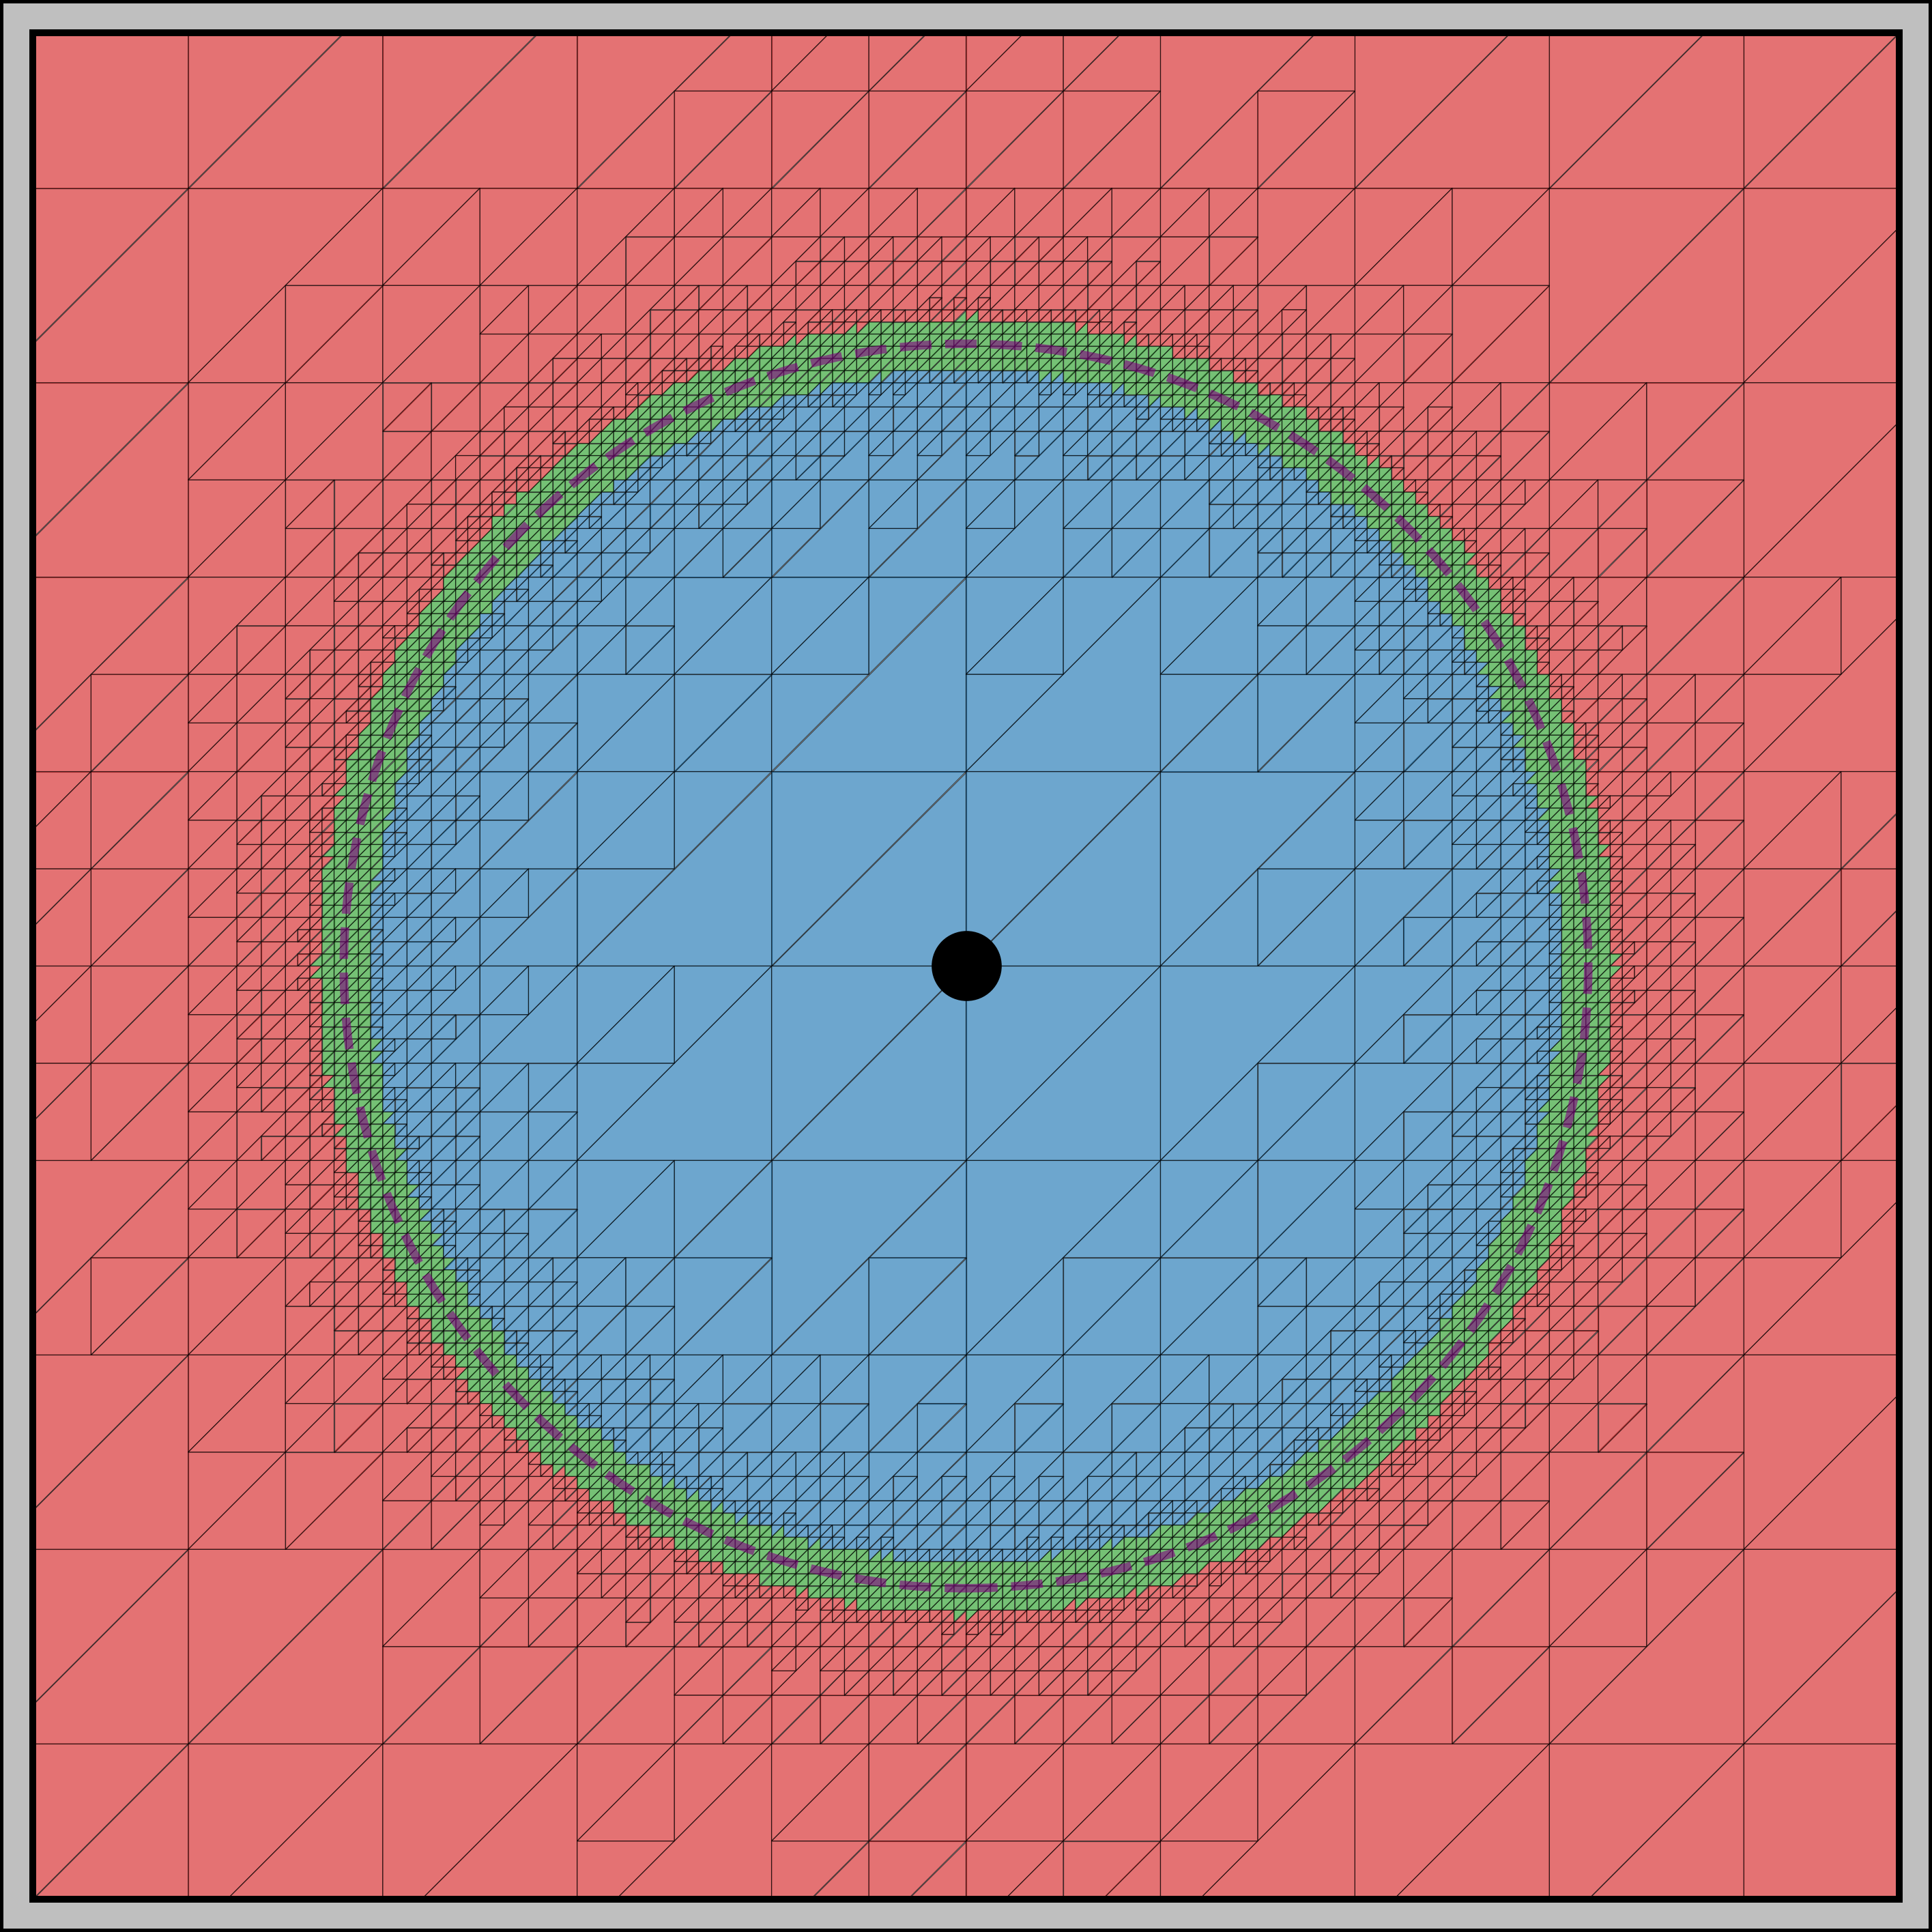
\includegraphics[width=\textwidth]{images/poisson_b2.png}
%     \end{minipage}
%     \label{dirac results}
% \end{figure}



% \begin{figure}[htbp]
%     \centering

%     % Main figure
%     \includegraphics[width=\textwidth]{images/poisson_b1.png}

 

%     % Bottom row: text on left, zoom on right
%     \begin{minipage}[c]{0.62\textwidth}
%         \small

%         \caption{Outer-refinement levels $k=0,3,6$ for
%         Algorithm~\ref{outerloop} applied to the
%         $\epsilon=0.2$ pseudospectrum of the Dirac-type operator
%         \eqref{dirac eig}. Black dots indicate the exact eigenvalues
%         \eqref{eigs dirac}. Red, blue, and green triangles are classified
%         as outside, inside, and on the pseudospectral contour,
%         respectively. White triangles outlined in grey remain active.
%        A magnified view of the $\mathcal{T}_6$ result over the region $[1.7,2.3]\times[-0.3,0.3]$ is shown to the right, with the desired contour indicated by the dashed purple circle.}
%         % Results from outer-refinement levels $k=0, 3, 6$ for Algorithm~\ref{outerloop} applied to the
%         % $\epsilon=0.2$ pseudospectrum of the Dirac-type operator \eqref{dirac eig}. Black dots indicate the exact eigenvalues \eqref{eigs dirac}. 
%         % Red, blue, and green triangles have been classified as outside, inside, and on the pseudospectral contour, respectively. The white triangles outlined in grey remain active. Since the green triangles are difficult to distinguish in the $\mathcal{T}_6$ result, a magnified view is shown to the right with the desired pseudospectral contour indicated by a dashed purple circle.
%         % outside the $\epsilon$-pseudospectrum, blue triangles as inside, green
%         % triangles as lying on the pseudospectral contour, and white triangles
%         % outlined in grey remain active. The resolution of the final sweep makes the green triangles hard to distinguish. We therefore present a magnified view with a purple dashed circle to indicate the desired pseudospectral contour.
%     \end{minipage}
%     \hfill
%     \begin{minipage}[c]{0.32\textwidth}
%         \centering
%         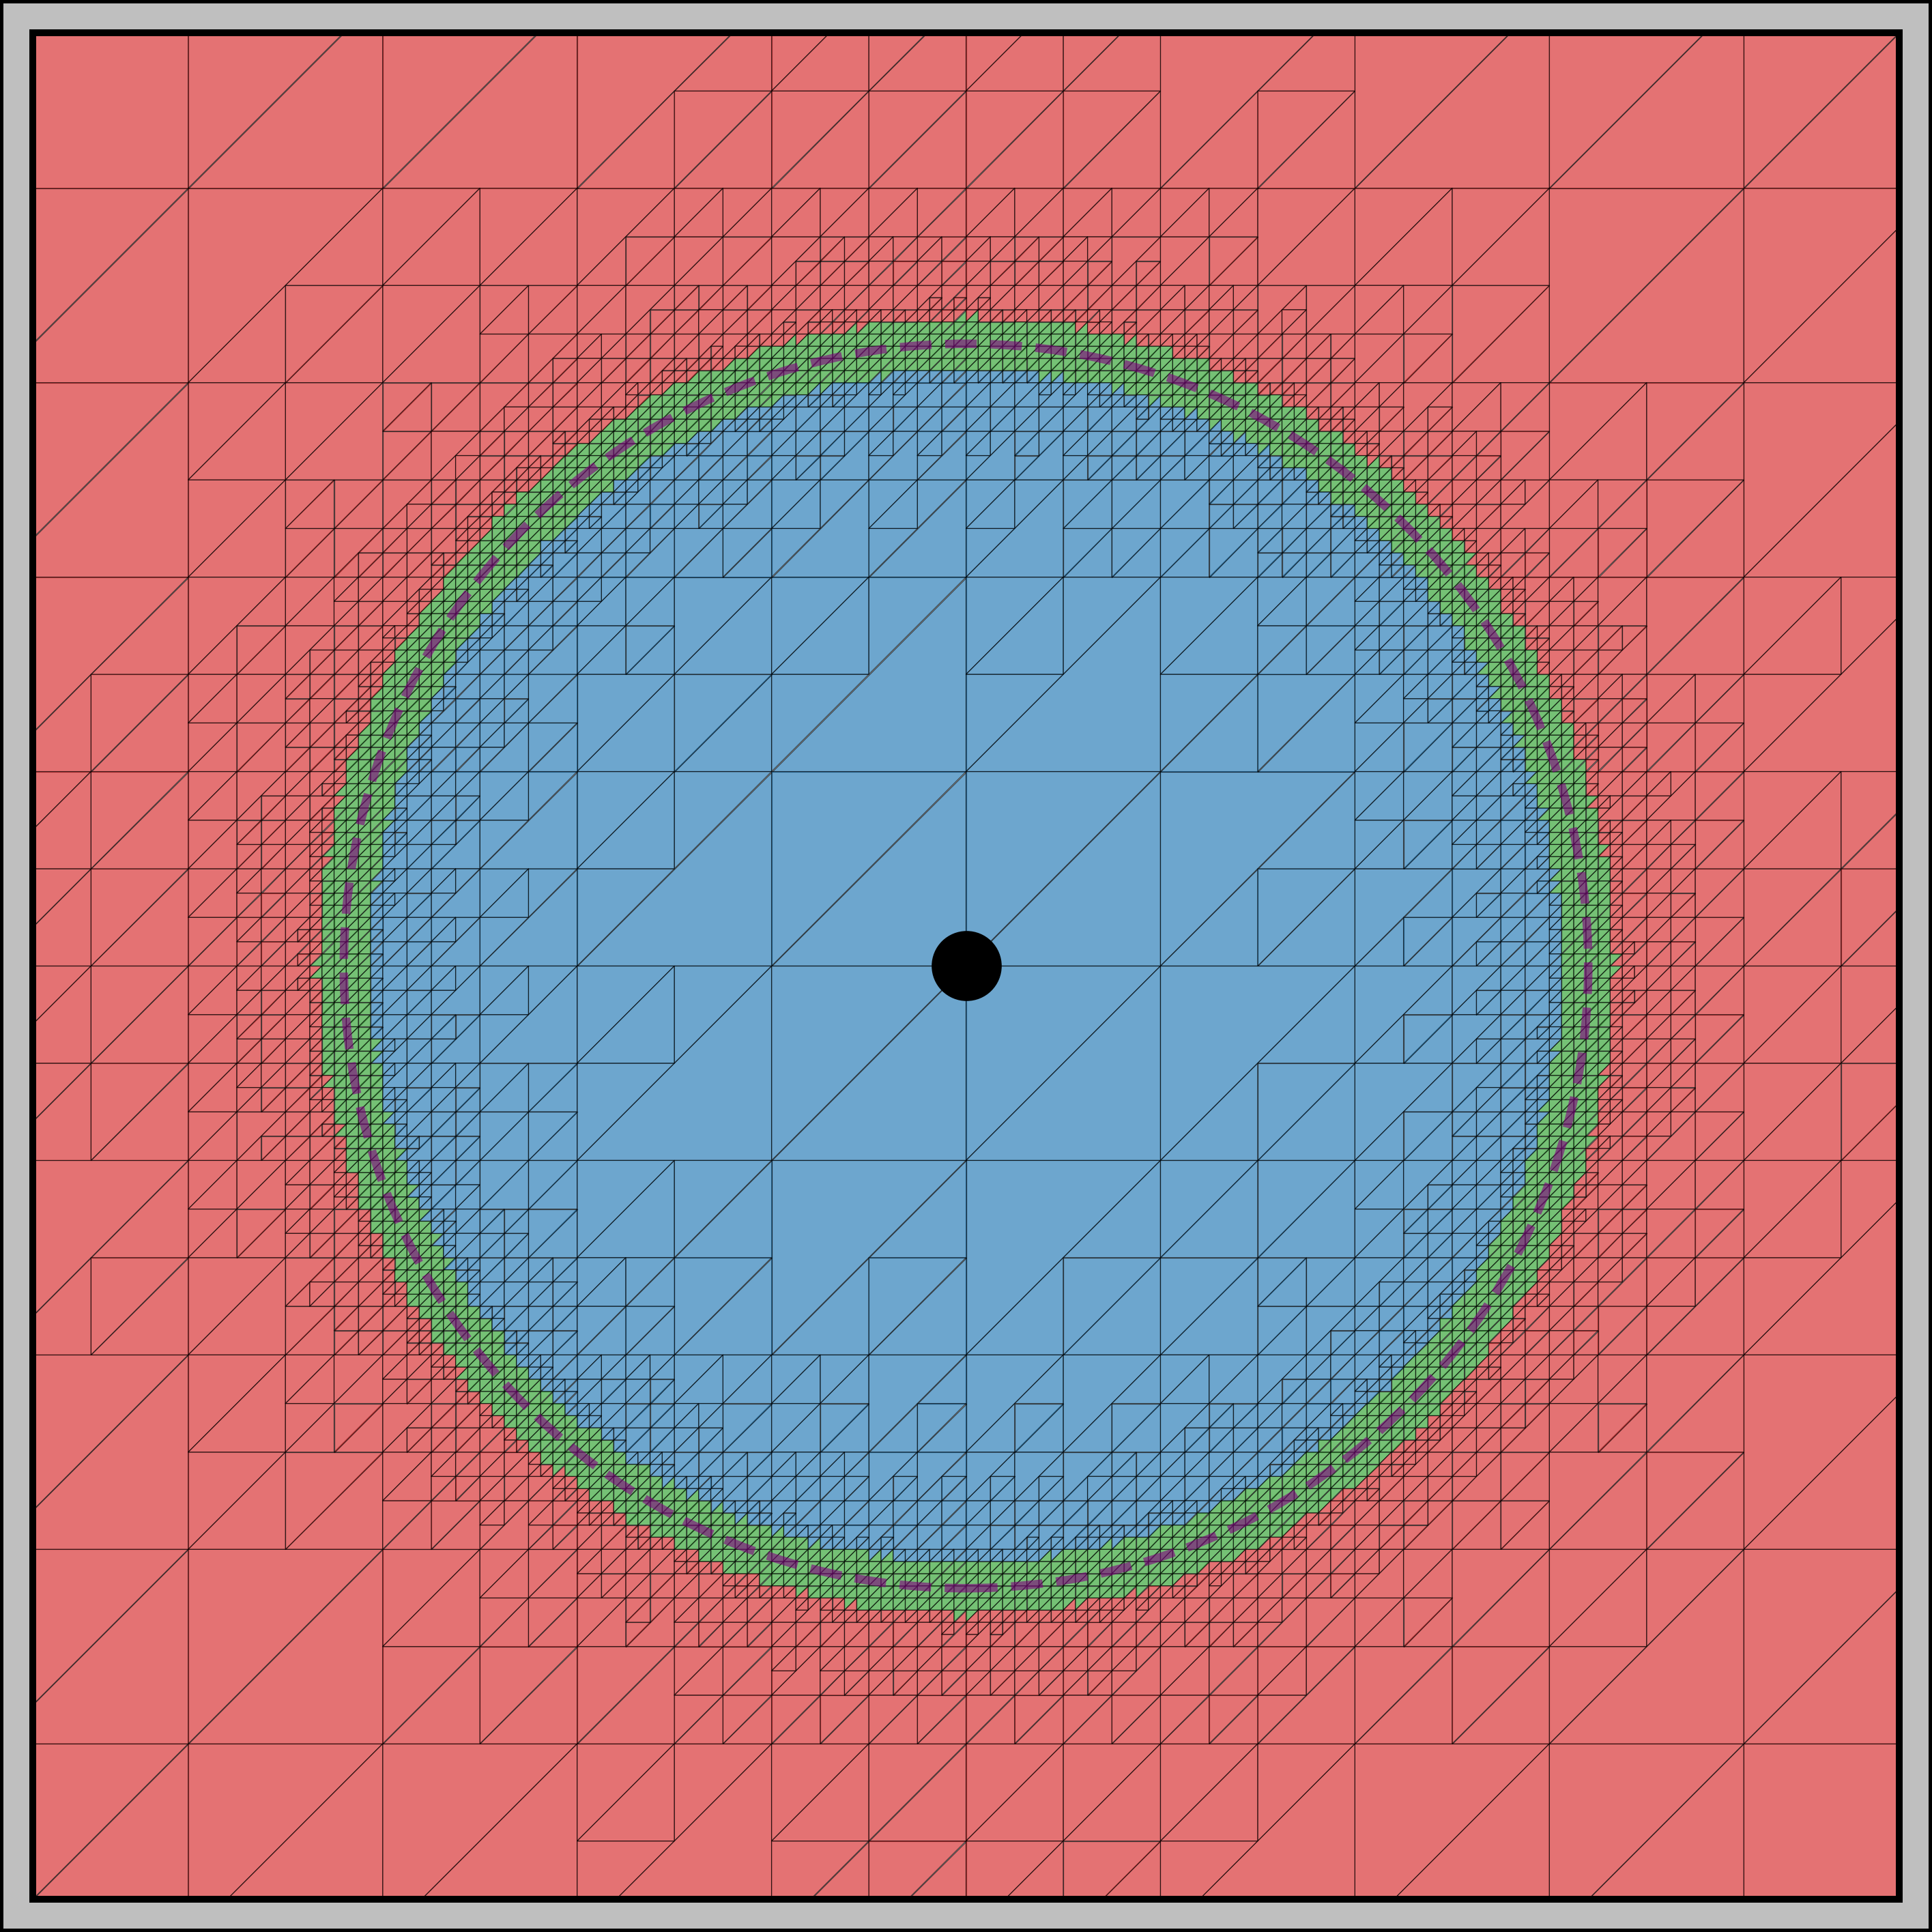
\includegraphics[width=\textwidth]{images/poisson_b2.png}
%     \end{minipage}
%     \label{dirac results}
% \end{figure}

% \begin{figure}[htbp]
%     \centering

%     % Main figure
%     \includegraphics[width=0.96\textwidth]{images/poisson_b1.png}

%     \vspace{0.3em}
% % Bottom row: caption on left, zoom on right
% \begin{minipage}[t]{0.69\textwidth}
%     \vspace{0pt}
%     \caption{
%         Outer-refinement levels $k=0,3,6$ for
%         Algorithm~\ref{outerloop} applied to the
%         $\epsilon=0.2$ pseudospectrum of the Dirac-type operator
%         \eqref{dirac eig}. Black dots indicate the exact eigenvalues
%         \eqref{eigs dirac}. Red, blue, and green triangles are classified
%         as outside, inside, and on the pseudospectral contour,
%         respectively; white triangles outlined in grey remain active.
%        A magnified view of the $\mathcal{T}_6$ result over the region $[1.7,2.3]\times[-0.3,0.3]$ is shown to the right, with the desired contour indicated by the dashed purple circle.
%     }
%     \label{dirac results}
% \end{minipage}
% \hfill
% \begin{minipage}[t]{0.27\textwidth}
%     \vspace{0pt}
%     \centering
%     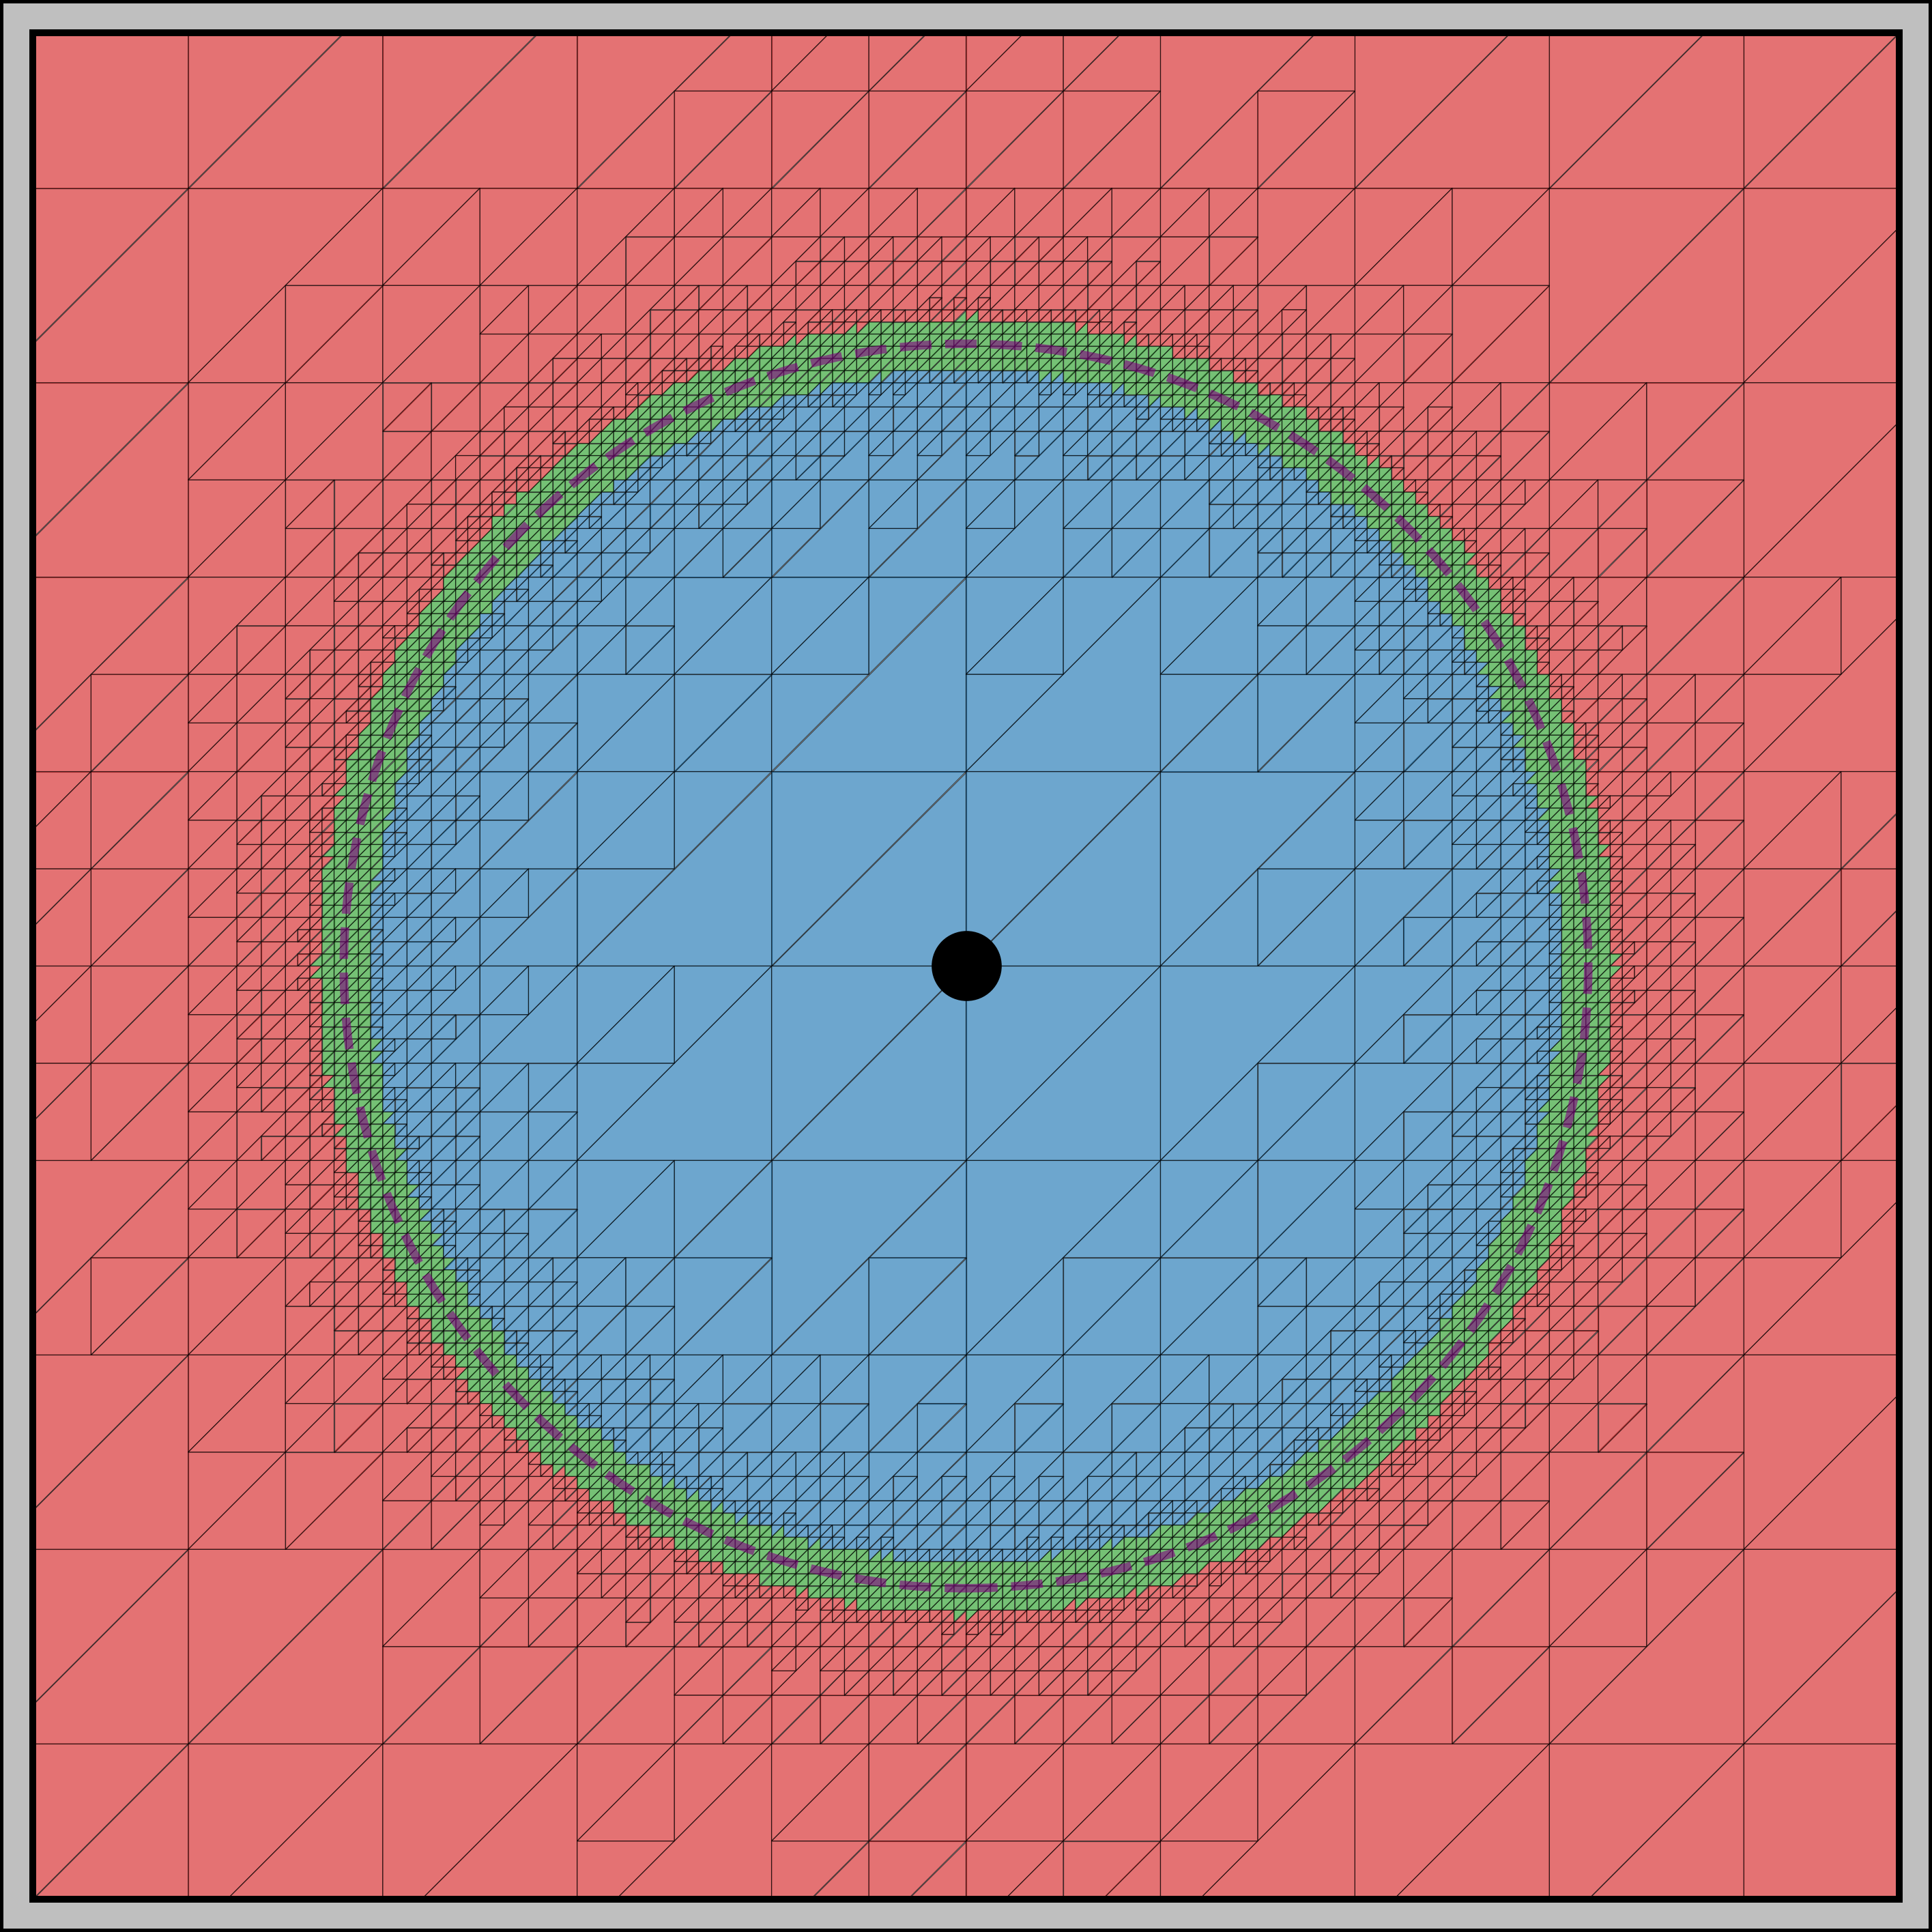
\includegraphics[width=\textwidth]{images/poisson_b2.png}
% \end{minipage}
% \end{figure}
